% pipeline.tex — Experimental pipeline sequential flow diagram
% Standalone TikZ figure; can also be \input{} into main.tex
% Compile: pdflatex pipeline.tex
\documentclass[tikz,border=4pt]{standalone}

\usepackage{tikz}
\usetikzlibrary{arrows.meta, positioning, shapes.geometric,
                calc, fit, backgrounds}

% ── Shared colour palette ────────────────────────────────────────────────────
\definecolor{StageBlue}    {RGB}{ 45, 105, 195}
\definecolor{StageBg}      {RGB}{215, 232, 255}
\definecolor{GRPOBlue}     {RGB}{ 30, 130, 200}
\definecolor{GRPOBg}       {RGB}{205, 238, 255}
\definecolor{PPOPurple}    {RGB}{120,  55, 185}
\definecolor{PPOBg}        {RGB}{235, 218, 255}
\definecolor{ArrowDark}    {RGB}{ 55,  60,  78}
\definecolor{NumberBg}     {RGB}{ 45, 105, 195}
\definecolor{BranchBg}     {RGB}{248, 248, 252}
\definecolor{BranchBorder} {RGB}{190, 198, 215}
\definecolor{WBGreen}      {RGB}{ 40, 160, 100}
\definecolor{WBBg}         {RGB}{218, 248, 232}

% ── Node styles ─────────────────────────────────────────────────────────────
\tikzset{
  % Numbered pipeline stage
  stage/.style={
    rectangle, rounded corners=5pt,
    fill=StageBg, draw=StageBlue, line width=0.85pt,
    font=\scriptsize\bfseries, text=StageBlue,
    inner sep=5pt, minimum width=1.65cm, minimum height=0.62cm,
    align=center
  },
  % Step number circle
  stepnum/.style={
    circle, fill=NumberBg, text=white,
    font=\tiny\bfseries,
    inner sep=0pt, minimum size=0.38cm
  },
  % GRPO branch node
  grponode/.style={
    rectangle, rounded corners=4pt,
    fill=GRPOBg, draw=GRPOBlue, line width=0.75pt,
    font=\tiny, text=GRPOBlue,
    inner sep=4pt, minimum width=2.1cm, minimum height=0.52cm,
    align=center
  },
  % PPO branch node
  pponode/.style={
    rectangle, rounded corners=4pt,
    fill=PPOBg, draw=PPOPurple, line width=0.75pt,
    font=\tiny, text=PPOPurple,
    inner sep=4pt, minimum width=2.1cm, minimum height=0.52cm,
    align=center
  },
  % W&B / logging node
  wbnode/.style={
    rectangle, rounded corners=4pt,
    fill=WBBg, draw=WBGreen, line width=0.75pt,
    font=\scriptsize\bfseries, text=WBGreen,
    inner sep=5pt, minimum width=1.65cm, minimum height=0.58cm,
    align=center
  },
  % Flow arrows (main pipeline)
  mainarrow/.style={
    ->, >=Stealth, line width=0.85pt, color=ArrowDark
  },
  % Branch arrows
  brancharrow/.style={
    ->, >=Stealth, line width=0.7pt
  }
}

% Helper: draw stage node + step number badge
% Usage: \Stage{node name}{number}{label text}{position spec}
\newcommand{\Stage}[4]{
  \node[stage, #4] (#1) {#3};
  \node[stepnum, above left=-0.14cm and -0.14cm of #1.north west] (#1_num) {#2};
}

\begin{document}
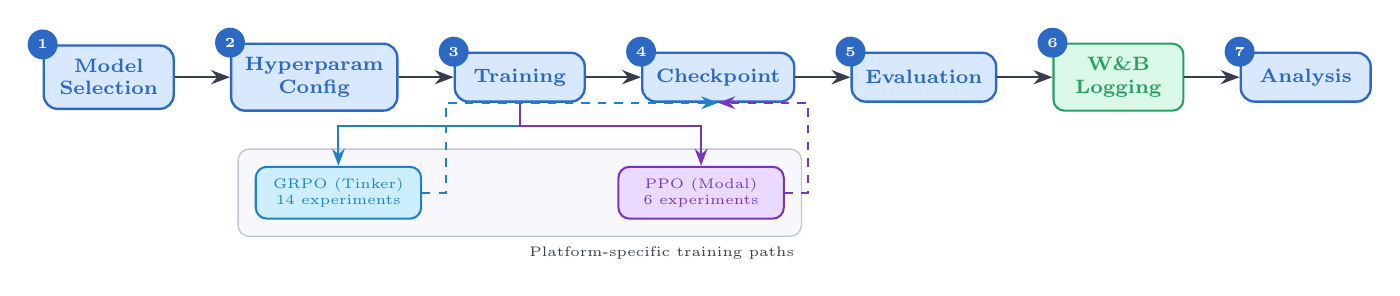
\begin{tikzpicture}[node distance=0.5cm and 0.42cm]

  % ── Main pipeline (7 stages) ──────────────────────────────────────────────

  % Stage 1: Model Selection
  \Stage{s1}{1}{Model\\Selection}{}

  % Stage 2: Hyperparameter Config
  \Stage{s2}{2}{Hyperparam\\Config}{right=0.7cm of s1}

  % Stage 3: Training (branch point — label only, no fill here; 
  %   actual branching handled below)
  \Stage{s3}{3}{Training}{right=0.7cm of s2}

  % Stage 4: Checkpoint
  \Stage{s4}{4}{Checkpoint}{right=0.7cm of s3}

  % Stage 5: Evaluation
  \Stage{s5}{5}{Evaluation}{right=0.7cm of s4}

  % Stage 6: W&B Logging
  \node[wbnode, right=0.7cm of s5] (s6) {W\&B\\Logging};
  \node[stepnum, above left=-0.14cm and -0.14cm of s6.north west] {6};

  % Stage 7: Analysis
  \Stage{s7}{7}{Analysis}{right=0.7cm of s6}

  % ── Main pipeline arrows ──────────────────────────────────────────────────
  \draw[mainarrow] (s1.east) -- (s2.west);
  \draw[mainarrow] (s2.east) -- (s3.west);
  \draw[mainarrow] (s3.east) -- (s4.west);
  \draw[mainarrow] (s4.east) -- (s5.west);
  \draw[mainarrow] (s5.east) -- (s6.west);
  \draw[mainarrow] (s6.east) -- (s7.west);

  % ── Branch: GRPO (Tinker) and PPO (Modal) paths below Stage 3 ────────────

  % GRPO node (left branch)
  \node[grponode, below left=0.8cm and 0.4cm of s3] (grpo_n)
        {GRPO (Tinker)\\14 experiments};

  % PPO node (right branch)
  \node[pponode, below right=0.8cm and 0.4cm of s3] (ppo_n)
        {PPO (Modal)\\6 experiments};

  % Arrows down from Training
  \draw[brancharrow, color=GRPOBlue]
        (s3.south) -- ++(0,-0.3) -| (grpo_n.north);
  \draw[brancharrow, color=PPOPurple]
        (s3.south) -- ++(0,-0.3) -| (ppo_n.north);

  % Arrows back up to Checkpoint
  \draw[brancharrow, color=GRPOBlue, dashed]
        (grpo_n.east) -- ++(0.3,0) |- (s4.south);
  \draw[brancharrow, color=PPOPurple, dashed]
        (ppo_n.east) -- ++(0.3,0) |- (s4.south);

  % ── Background panel for branch area ─────────────────────────────────────
  \begin{scope}[on background layer]
    \node[rectangle, rounded corners=4pt,
          fill=BranchBg, draw=BranchBorder, line width=0.5pt,
          fit=(grpo_n)(ppo_n), inner sep=6pt] {};
  \end{scope}

  % ── Branch label ──────────────────────────────────────────────────────────
  \node[font=\tiny, text=ArrowDark, below=0.22cm of ppo_n,
        xshift=-0.5cm, align=center]
        {Platform-specific training paths};

\end{tikzpicture}
\end{document}
